\chapter{Related Works}
In this chapter we review the main challenges in the application of reinforcement learning in the
field of robotics. The majority of this information is derived from \cite{Kober2013}.

\section{Reinforcement Learning in Robotics}

\subsubsection{Curse of Dimensionality}
Robotics systems often have to deal with high dimensional states and actions due to the many degrees of freedom (DoFs) of modern
anthropomorfic robots. For example, in the ball-paddling task shown in Figure \ref{fig:ball_paddling_robot}, a proper representation
of a robot's state would consist of its joint angles and velocities for each of its seven DoFs as well as the cartesian position
and velocity of the ball. The robot's actions would be the generated motor commands, which often are torques or accelerations.
In this example, we have $2\times\left(7 + 3\right)=20$ state dimensions and 7-dimensional continuous actions.

This high dimensionality presents significant challenges in terms of computational complexity 
and the efficiency of learning algorithms.

\begin{figure}[b]
    \centering
    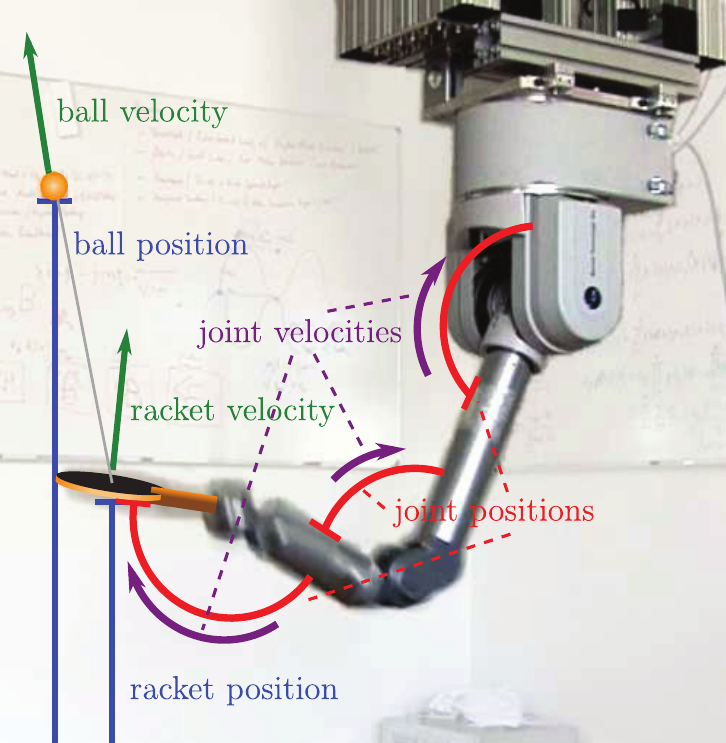
\includegraphics[width=0.3\textwidth]{Images/ball_paddling.png}
    \caption{Ball Paddling Robot}
    \label{fig:ball_paddling_robot}
\end{figure}

This problem is solved with function approximators like neural networks using Deep Reinforcement Learning algorithms.

\subsubsection{Curse of real-world samples}
Robots interact with the physical world, hence robot reinforcement learning suffers from most of the resulting real-world problems.
For example, robot hardware is usually expensive, suffers from wear and tear, and requires careful maintenance. This is why safe exploration
becomes a key issue in the learning process.

Several more aspects of the real-world make robotics a challenging domain. Frequently, the environment settings during an earlier 
learning period cannot be reproduced. This problem makes comparing algorithms particularly hard. Furthermore, the approaches often have to deal 
with uncertainty due to inherent measurement noise and the inability to observe all states directly with sensors.

Most real robot learning tasks require some form of human supervision, e.g. putting the pole back on the robot's end-effector during pole balancing
 after a failure. Even when an automatic reset exists, the learning speed becomes essential as a task on a real robot cannot be sped up.
In some tasks such as a slowly rolling robot, the dynamics can be ignored; in others such as a flying robot, they cannot. In particular in the latter case,
often the whole episode needs to be completed as it is not possible to start from arbitrary states.

For such reasons, real-world samples are expensive in terms of time, labor and, potentially, finances. In robotic reinforcement learning,
it is often considered to be more important to limit the real-world interaction time instead of limiting memory consumption or computational complexity.
Thus, sample efficient algorithms that are able to learn from a small number of trials are essential.

Since the robot is a physical system, there are strict constraints on the interaction between the learning algorithm
and the robot setup. For dynamic tasks, the movement cannot be paused and actions must be selected within a time-budget without 
the opportunity to pause to think, learn or plan between actions.

As reinforcement learning algorithms are inherently implemented on a digital computer, the discretization of
time is unavoidable despite that physical systems are inherently continuous time systems. Time-discretization of the
actuation can generate undesirable artifacts (e.g. the distortion of distance between states) even for idealized physical
systems, which cannot be avoided. As most robots are controlled at fixed sampling frequencies (in the range between
500 Hz and 3 kHz) determined by the manufacturer of the robot, the upper bound on the rate of temporal discretization
is usually pre-determined. The lower bound depends on the horizon of the problem, the achievable speed of changes in
the state, as well as delays in sensing and actuation. All physical systems exhibit such delays in sensing and
actuation. The state of the setup (represented by the filtered sensor signals) may frequently lag behind the real state due
to processing and communication delays. More critically, there are also communication delays in actuation as well
as delays due to the fact that neither motors, gear boxes nor the body's movement can change instantly. Owing to
these delays, actions may not have instantaneous effects but are observable only several time steps later. In contrast, 
in most general reinforcement learning algorithms, the actions are assumed to take effect instantaneously as such
delays would violate the usual Markov assumption. This effect can be addressed by putting some number of recent
actions into the state. However, this significantly increases the dimensionality of the problem.
The problems related to time budgets and delays can also be avoided by increasing the duration of the time steps.
One downside of this approach is that the robot cannot be controlled as precisely; another is that it may complicate a
description of system dynamics.

\subsubsection{Curse of under-modeling and model uncertainty}
One way to offset the cost of real-world interaction is to use accurate models as simulators. In an ideal setting, this
approach would render it possible to learn the behavior in simulation and subsequently transfer it to the real robot.
Unfortunately, creating a sufficiently accurate model of the robot and its environment is challenging and often requires
very many data samples. As small model errors due to this under-modeling accumulate, the simulated robot can
quickly diverge from the real-world system.

Fot tasks where the system is self-stabilizing (that is, where the robot does not require active control to remain in a safe state or return to it),
transferring policies often works well. Nevertheless, tasks can often be learned better in the real world than in simulation due to complex mechanical interactions
that have proven difficult to model accurately. In contrast, in unstable tasks small variations have drastic consequences. For example, in a pole balancing
task, the equilibrium of the upright pole is very brittle and constant control is required to stabilize the system. Transferred policies often perform poorly
in this setting.

\subsubsection{Curse of goal specification}
In reinforcement learning, the desired behavior is implicitly specified by the reward function. The goal of reinforcement
learning algorithms then is to maximize the accumulated long-term reward. While often dramatically simpler than
specifying the behavior itself, in practice, it can be surprisingly difficult to define a good reward function in robot
reinforcement learning. The learner must observe variance in the reward signal in order to be able to improve a
policy: if the same return is always received, there is no way to determine which policy is better or closer to the
optimum. In many domains, it seems natural to provide rewards only upon task achievement, for example, when a table tennis
robot wins a match. This view results in an apparently simple, binary reward specification. However, a robot may
receive such a reward so rarely that it is unlikely to ever succeed in the lifetime of a real-world system. Instead of
relying on simpler binary rewards, we frequently need to include intermediate rewards in the scalar reward function
to guide the learning process to a reasonable solution, a process known as \textit{reward shaping} \cite{Laud2004}.

\section{Robot Reinforcement Learning on the Constraint Manifold}
One important factor that cannot be neglected in real-world applications is the necessity of satisfying constraints.
Many practical considerations can be formulated in the form of constraints, such as safety and mechanical viability. For example,
in the robot manipulation task, the robot should not take actions that damage the environment and cannot take actions that exceed
its feasible range.

In order to achieve safe exploration during learning process in continuous control problems different algorithms have been developed.
This section describes one of them, called ATACOM \cite{Atacom}.
 
ATACOM transforms a constrained RL problem into a typical unconstrained RL problem. Hence the problem can be addressed by any
model-free RL algorithm while maintaining the constraints below the tolerance. Furthermore, ATACOM can handle both equality and inequality
constraints.

The advantages of ATACOM can be summarized as follows:
\begin{itemize}
    \item It can deal both with \textbf{equality and inequality constraints}. All of the constraints at each time step are maintained
    below the tolerance during the whole process.
    \item It does not require an initial feasible policy, the agent can \textbf{learn from scratch}.
    \item It requires \textbf{no manual safe backup policy} to move the system back into the safe region.
    \item It can be applied to any model-free RL algorithm, using both \textbf{deterministic and stochastic policies}
    \item It can focus the exploration on the \textbf{lower-dimensional manifold} instead of exploring in the original action space
    for equality constrained problem.
    \item It has \textbf{better learning performance} as the inequality constraints restrict to a smaller feasible state-action space.
\end {itemize}

As a downside this method requires
\begin{itemize}
    \item differentiable constraint functions.
    \item a sufficiently accurate invertible dynamics model of the robot or a well-performed tracking controller.
\end{itemize}

% \begin{definition}
%     A Constrained Markov Decision Process (CMDP) is a tuple $(\mc{S}, \mc{A}, P, R, \gamma, \mc{C})$, where $\mc{S}$ is a state-space,
%     $\mc{A}$ is an action space, $P: \mc{S}\times\mc{A}\times\mc{S} \to [0,1]$ is a transition kernel, $\gamma$ is a discount factor,
%     and $\mc{C}: \left{c_i : \mc{S} \to \mathbb{R} | i \in 1, \dots, k}$ is a set of \textit{immediate state-constraint} functions.
% \end{definition}

% The state variable $s \in \mc{S}$ is decomposed in the directly controllable state $q \in \mc{Q}$ and uncontrollable state 


